\chapter{Ein Kapitel}
\section{Eine Sektion}
\label{sec:first-section}

\begin{align*}
  \cee{Cl2 &-> 2 Cl} \reactiontag\\
  \cee{Cl + CH4 &-> HCl + CH3} \\
  \cee{CH3 + Cl2 &-> ClCH3 + Cl}
\end{align*}

\begin{align*}
  \reactione[rxn1]{Cl2 &-> 2 Cl}\\
  \reactione[rxn2]{Cl + CH4 &-> HCl + CH3} \\
  \reactione[rxn3]{CH3 + Cl2 &-> ClCH3 + Cl}
\end{align*}

Referenztest:
Eine Reaktion \ref{rxn1} oder noch eine Reaktion \ref{rxn3}. 

Ein wenig Blindtext: 
Lorem ipsum dolor sit amet, consectetuer adipiscing elit. Aenean commodo ligula eget dolor. Aenean massa. Cum sociis natoque penatibus et magnis dis parturient montes, nascetur ridiculus mus. Donec quam felis, ultricies nec, pellentesque eu, pretium quis, sem. Nulla consequat massa quis enim. Donec pede justo, fringilla vel, aliquet nec, vulputate eget, arcu. In enim justo, rhoncus ut, imperdiet a, venenatis vitae, justo. Nullam dictum felis eu pede mollis pretium. Integer tincidunt. Cras dapibus. Vivamus elementum semper nisi. Aenean vulputate eleifend tellus. Aenean leo ligula, porttitor eu, consequat vitae, eleifend ac, enim. Aliquam lorem ante, dapibus in, viverra quis, feugiat a, tellus. Phasellus viverra nulla ut metus varius laoreet. Quisque rutrum. Aenean imperdiet. Etiam ultricies nisi vel augue. Curabitur ullamcorper ultricies nisi. Nam eget dui. Etiam rhoncus.

Man kann Text auch \emph{hevorheben}. 

\subsection{Eine Untersektion}
Lorem ipsum dolor sit amet, consectetuer adipiscing elit. Aenean commodo ligula eget dolor. Aenean massa. Cum sociis natoque penatibus et magnis dis parturient montes, nascetur ridiculus mus. Donec quam felis, ultricies nec, pellentesque eu, pretium quis, sem. Nulla consequat massa quis enim. Donec pede justo, fringilla vel, aliquet nec, vulputate eget, arcu. In enim justo, rhoncus ut, imperdiet a, venenatis vitae, justo. Nullam dictum felis eu pede mollis pretium. Integer tincidunt. Cras dapibus. Vivamus elementum semper nisi. Aenean vulputate eleifend tellus. Aenean leo ligula, porttitor eu, consequat vitae, eleifend ac, enim. Aliquam lorem ante, dapibus in, viverra quis, feugiat a, tellus. Phasellus viverra nulla ut metus varius laoreet. Quisque rutrum. Aenean imperdiet. Etiam ultricies nisi vel augue. Curabitur ullamcorper ultricies nisi. Nam eget dui. Etiam rhoncus.


\chapter{Ein zweites Kapitel}
\section{Einige Beispiele zur Mathematik, Graphiken und Tabellen}
Man kann auf Dinge verweisen, beispielweise auf Sektion \vref{sec:first-section}.

Es gibt einfache, fließende Graphiken wie beispielsweise Abbildung \ref{fig:ionMigSim-experiment-overview}. 

\begin{figure}[tb]
   \begin{center}
   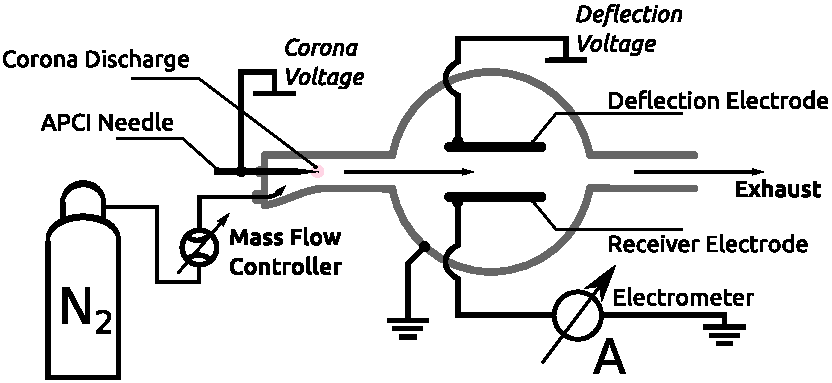
\includegraphics[width=0.8\columnwidth]{images/ionMigration_experimentOverview.pdf}
   \caption[Schematic benchmark overview]{Schematic overview of the benchmark experiment. Nitrogen gas flows trough the ion source and the measurement chamber. Ions are generated upstream by a corona discharge. The ions are transported into the measurement chamber by the bulk gas flow. Here, a potential on the deflection electrode pushes the ions on the receiver electrode. The ion current on the receiver electrode is measured in dependence of the gas flow and the deflection potential.}
   \label{fig:ionMigSim-experiment-overview}
   \end{center}
\end{figure}

Es gibt auch komplexere Graphiken bzw. fließende Objekte. Zum Beispiel Abbildung \ref{fig:nebuPos_01_nebuPosVari}. Man kann auch Tabellen einbauen, wie zum Beispiel Tabelle \vref{tab:ionMigSim-fluidparameters}. Manchmal muss man auch was zitieren \cite{Poehler2011}, manchmal auch mehr \cite{Serway2009,Chang1991} und noch mehr \cite{Valentine2009,Schiewek2007,Python2.7}.

\begin{table}
\caption{Parameters of the bulk gas flow simulation}
\label{tab:ionMigSim-fluidparameters}
\begin{center}
  \begin{tabulary}{\textwidth}{LL} 
		static temperature & $T=\unit[298.15]{K}$ \\
		background pressure & $p=\unit[1.01\cdot 10^{5}]{Pa}$ \\
		mean outflow velocity & $v_{out} = \unit[0.15 - 1.35]{m/s}$ \\
 		gas density & $\rho= \unit[1.164]{kg/m^3}$ \\ 
     	dynamic viscosity & $\mu= \unit[1.744\cdot 10^{-5}]{Pa\cdot s}$ \\ 
  \end{tabulary}
\end{center}
\end{table}

\begin{sidewaysfigure}
	\begin{center}
   		\begin{subfigure}{0.45\columnwidth}
   			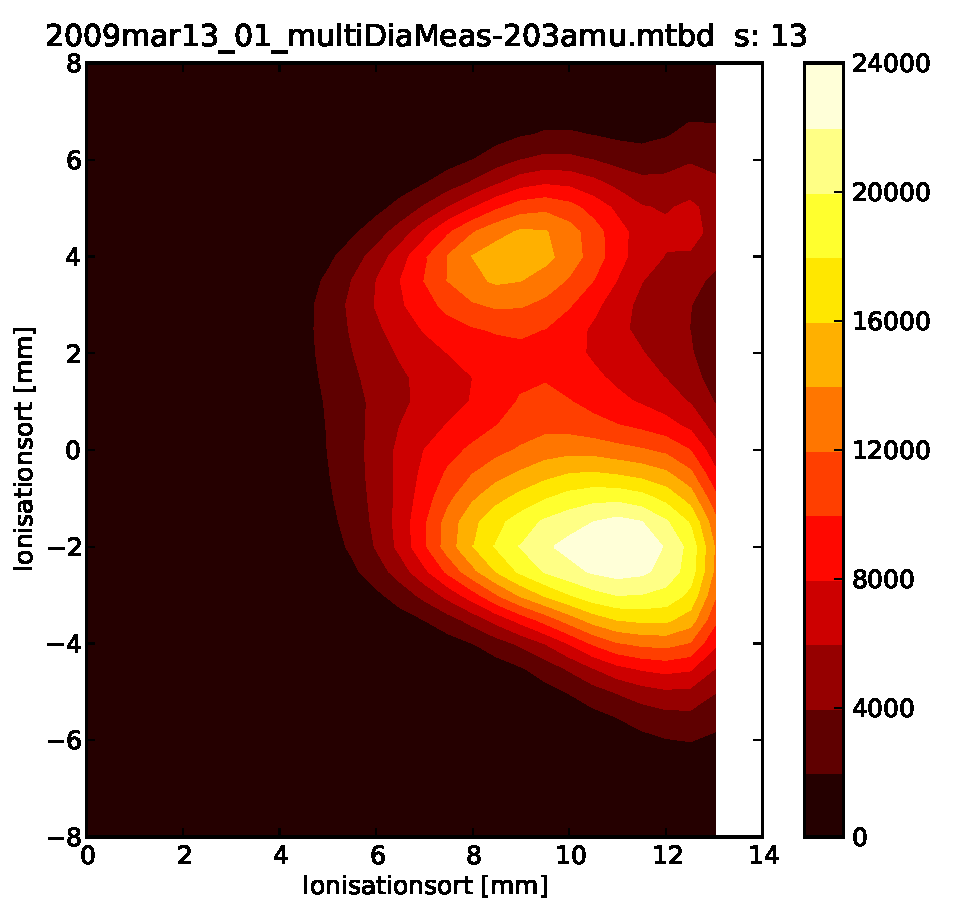
\includegraphics[width=1\columnwidth]{images/nebuPos_01_2000_50_2l_1_9mm.pdf} 
			\caption{Neb.-Pos.: \unit[17,7]{mm}}
			\label{nebuPos_01_17.7}
		\end{subfigure}
		\begin{subfigure}{0.45\columnwidth}
   			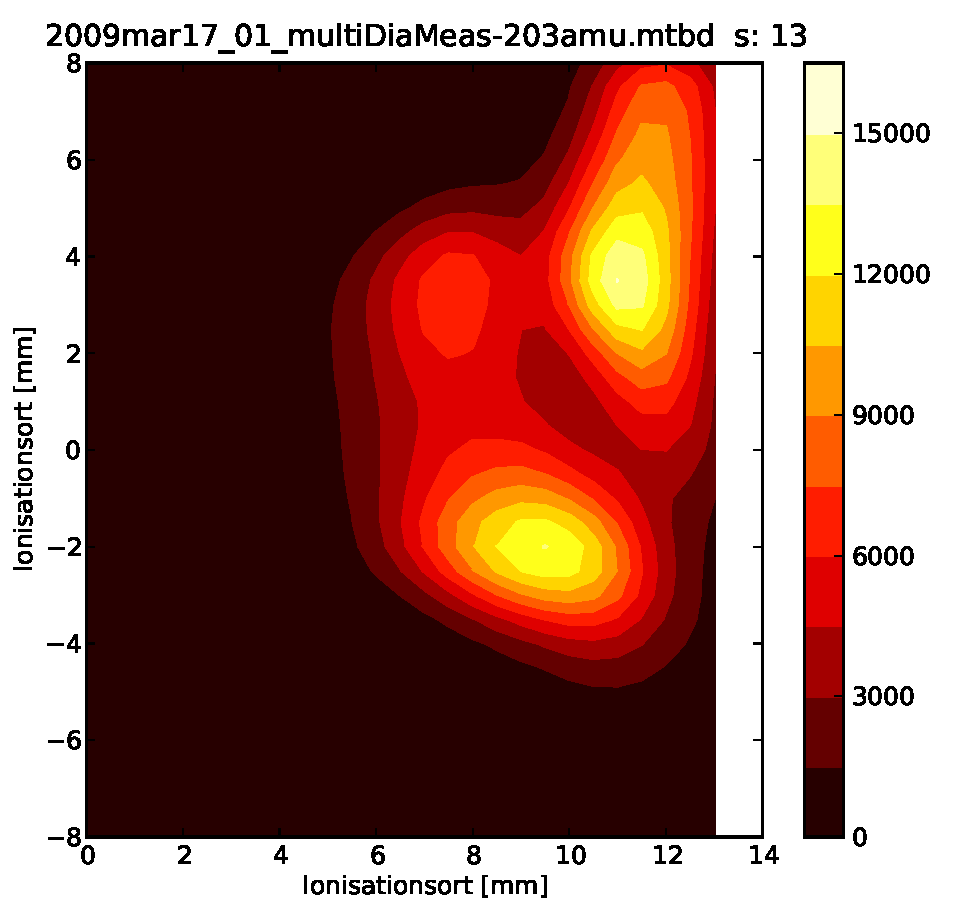
\includegraphics[width=1\columnwidth]{images/nebuPos_01_2000_50_2l_4_2mm.pdf} 
			\caption{Neb.-Pos.: \unit[13,5]{mm}}
			\label{nebuPos_01_17.7}
		\end{subfigure}
   		\caption[Variation der Nebulizer-Position]{Variation der Nebulizer-Position, bei einer Kapillar-Spannung von \SI{-2000}{V}, einer Sprayshield-Spannung von \SI{-50}{V} und einem Drygas-Fluss von \SI{2,0}{l min^{-1}} }
   		\label{fig:nebuPos_01_nebuPosVari}
   \end{center}
\end{sidewaysfigure} 

Man kann auch mathematische Symbole benutzen im Fließtext, beispielsweise ist $\lambda$ ein oft in der Mathematik verwendeter griechischer Buchstabe. Es gilt auch weiterhin $\pi \approx 3.14$. 

Man kann aber auch numerierte Gleichungen setzen: 
\begin{equation}
c^2 = a^2 + b^2
\end{equation}

oder auch Komplizierteres, wie Folgendes beispielsweise: 

The momentum equations in the three spatial dimensions $(x,y,z)$ are: 
\begin{eqnarray}
\frac{\partial(\rho u)}{\partial t}+\nabla\cdot(\rho u \mathbf{u}) & = -\frac{\partial p}{\partial x} + \nabla\cdot(\mu \nabla u) + S_{m_x} \\
\frac{\partial(\rho v)}{\partial t}+\nabla\cdot(\rho v \mathbf{u}) & = -\frac{\partial p}{\partial y} + \nabla\cdot(\mu \nabla v) + S_{m_y} \\ 
\frac{\partial(\rho w)}{\partial t}+\nabla\cdot(\rho w \mathbf{u}) & = -\frac{\partial p}{\partial z} + \nabla\cdot(\mu \nabla v) + S_{m_z} 
\end{eqnarray}

oder auch 

\begin{equation}\label{eqn:avg-viscous-damping-function}
f(t) = \frac{1-e^{-k_0 \delta t}} {\delta t k_0}
\end{equation}

Als Chemiker setzt man auch oft chemische Formeln, was mit dem mhChem Paket ganz vorzüglich gelingt. Ein Beispiel für eine inline formel ist \ce{A -> P}, eine Reaktion eines Ausgangsstoffes \ce{A} zu einem Produkt \ce{P}.

Wir haben uns auch eine eigene Umgebung für Reaktionen, mit einem eigenen Zähler definiert im Master-Dokument, die man so verwenden kann: 
\reaction[rxn:knallgas-reaktion]{2H2 + O2 -> 2H2O}
Das mhchem Paket kann auch mit Ionen umgehen. Bei der Elektronenstoßionisation passiert beispielsweise Folgendes: 
\reaction[rxn:EI-ionization]{M + e^- -> M^{+.} + 2e^-}

